\documentclass[12pt]{article}
\usepackage{fullpage,url,amssymb,epsfig,color,xspace,amsmath}
\usepackage{graphicx}
\usepackage{biblatex}
\usepackage{bbm}
\usepackage{slashbox}
\usepackage[]{algorithm2e}
\usepackage{pgfplots} % bar graphs
\usepackage{setspace}
\usepackage{tikz} %draw fancy pictures
\usepackage{verbatim}
\usetikzlibrary{calc,matrix}
\usepackage{caption}
\usepackage{amssymb}
\usepackage{amsmath}
\usepackage{amsthm}
\usepackage{graphicx}
\usepackage{mathtools}
\usepackage{enumitem}
\setlist{noitemsep} %set line separation of items to zero
\setlength\parindent{0pt} %no automatic indentation for new paragraph
\usetikzlibrary{arrows,shapes}
\usepackage{hyperref}
\usetikzlibrary{calc}
\setlength\parindent{0pt}
\usetikzlibrary{shapes.geometric}
\pgfplotsset{width=10cm,compat=1.8}
\newcommand{\pmtn}{\text{pmtn}}
\newcommand{\Note}{\paragraph{Note:}}
\newcommand{\Definition}{\paragraph{Definition}}
\newcommand{\Question}{\paragraph{Question}}
\newcommand{\Example}{\paragraph{Example}}
\newcommand{\Problem}{\paragraph{Problem}}
\newcommand{\Theorem}{\paragraph{Theorem}}
\newcommand{\tabfour}{\hspace*{100pt}}
\newcommand{\tabthree}{\hspace*{75pt}}
\newcommand{\tabtwo}{\hspace*{50pt}}
\newcommand{\tab}{\hspace*{25pt}}
\newcommand{\ra}{\rightarrow}
\newcommand{\Ra}{\Rightarrow}
\newcommand{\la}{\leftarrow}
\hypersetup{
	colorlinks=true, %set true if you want colored links
	linktoc=all,     %set to all if you want both sections and subsections linked
	linkcolor=blue,  %choose some color if you want links to stand out
}
\begin{document}
	
	\begin{center}
		\vspace*{3cm}	
		\textbf{\LARGE John Forbes Nash - First Edition}\\
		\vspace{5pt}
		\large Michael Ryan Blair, Xin Ye Liu, Mohammed Tahir Zaman, Brandon Yeh\\
		\vspace{5pt}
		CO480 - Spring 2015\\
	\end{center}
	
	\newpage
	
	\tableofcontents
	
	\newpage
	
	\singlespacing
	
	\section{Introduction to Game Theory \& Strategic Games}
	The creation of the field of Game Theory is largely attributed to John von Neumann and Oskar Morgenstern who fully introduced the concepts of cooperative games and 2-player zero-sum games in their paper \cite{1} . This exposition was published in 1944 and built on works published by the two authors dating back to 1928 \cite{2}. This work provided a new approach to a number of problems in economics. \\
	
	Since this early work, the field of Game Theory has exploded. Game Theory has is used to study and explain phenomena not only in economics, but also in military tactics, biology, and in real-world corporate business decisions (e.g. Mergers \& Acquisitions, pricing decisions, supplier negotiations).
	
	\section{Strategic Games}
	
	We first define the class of games that Nash, and subsequently this paper will study. For the purposes of this paper, strategic games are games with N players, each of which has a finite number of pure strategies. This induces the following notation and definitions.
	
	\subsection{Definitions \& Notation}
	
	\Definition A strategic game with $N$ players has \textbf{player set} $\{1,...,n\}$ denoted by $N$\\
	
	Each player $i \in N$ has a finite number of pure strategies. The set of all of player i's strategies is denoted as $S_i$, and an individual pure strategy is denoted as $s_i$.\\
	
	A strategy profile denoted $S$ is a N-tuple, where each element $i$ is a pure strategy of player $i$.\\
	
	The collection of all strategy profiles $S$ is denoted as $\mathbb{S}$. We have then 
	\begin{equation*}
	\mathbb{S} = S_1 \times S_2 \times \cdots \times S_n
	\end{equation*} where $\times$ represents the Cartesian product of sets.\\
	
	We also define the following utility/payoff functions.
	
	\begin{equation*}
	\forall i, u_i : \mathbb{S} \Rightarrow \mathbb{R}
	\end{equation*}
	
	Each of the $u_i$ takes in a strategy profile and returns the utility value that the player receives under the strategy profile $S$. That is, if each player $i$ plays the strategy $s_i$ in S, the player $i$ will receive a payoff of $u_i(S)$
	
	\Note The specific payoff amount may have no meaning in a strategic game. The only claim is that a player prefers a higher payoff to a smaller payoff. We cannot, however, say that a player prefers a payoff of 2, twice as much as a payoff of 1.\\
	
	We also introduce the following substitution notation:\\
	
	Suppose $S = (s_1,...,s_n)$. Then the strategy profile $(S_{-i},s_i') = (s_i,...,s_{-1},s_i',s_{i+1},...,s_n)$. In words, $(S_{-1},s_i')$ is the strategy profile obtained from S when player $i$ changes their strategy from $s_i$ to $s_i'$\\
	
	\subsection{How are Strategic Games Played?}
	In strategic games each player moves simultaneously. That is, each player selects a strategy at the same time, and each players' strategy selection is independent of the strategies chosen by the other players. Each player then receives payoff $u_i(S)$ based on the actions of each player.\\
	
	We make two key assumptions when playing strategic games:
	\begin{enumerate}
		\item Each player is a rational actor with the single goal of maximizing their own utility, meaning that a player will always choose the action that, given the other player's strategies - will yield the highest payoff.\\
		
		\item We assume that players have played these games extensively in the past. It is assumed that this has led each player to form beliefs about how their opponents will play the game. This assumption is applied to each player, and it is assumed that all such beliefs are consistent.
	\end{enumerate}
	
	\subsection{Examples of Strategic Games}
	To illustrate strategic games, two-player games are often given in matrix form. The rows correspond to each of player 1's moves, and the columns correspond to player 2's moves. The elements of the matrix are ordered pairs (x, y) where x and y are the payoffs to player 1 and 2 respectively. 
	
	\newpage
	\paragraph{Prisoner's Dilemma\\}
	
Set-up: Two prisoners have been captured and are being interrogated about their involvement with a crime. Each prisoner has two options: remaining quiet (Q), or confessing (C). If both prisoners remain quiet, the police can only convict them of a minor charge. If both prisoners confess, the police will convict them of a major charge, but the sentence will be reduced because of their cooperation. If one prisoner confesses, they will go free and their accomplice will be convicted of the major offence. This situation can be modelled as the following strategic game:
	\begin{center}
	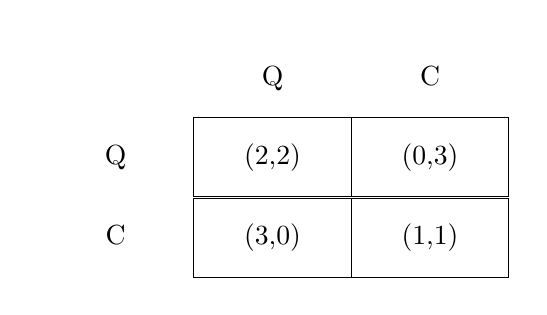
\begin{tikzpicture}[element/.style={minimum width=2cm,minimum height=1cm}]
	\matrix (m) [matrix of nodes,nodes={element},column sep=-\pgflinewidth, row sep=-\pgflinewidth,]{
		& Q  & C  \\
		Q & |[draw]|(2,2) & |[draw]|(0,3) \\
		C & |[draw]|(3,0) & |[draw]|(1,1) \\
	};
	
	\end{tikzpicture}
\end{center}

This results in the following instances of our definitions:
\begin{itemize}
	\item $\mathbb{S} = \{(Q,Q),(Q,C),(C,Q),(C,C)\}$
	\item $S_1 = S_2 = \{Q,C\}$
	\item $u_1((Q,Q)) = 1$
	\item $u_2((C,Q)) = 0$
\end{itemize}

\paragraph{Matching Pennies\\}

Set-up: Two players are each holding a penny. They each choose to show either Heads (H) or Tails (T). If both players select the same side, Player 2 pays player 1 \$1. If the sides do not match, then player 1 pays player 2 \$1.
This can be represented by the following matrix form:
\begin{center}
	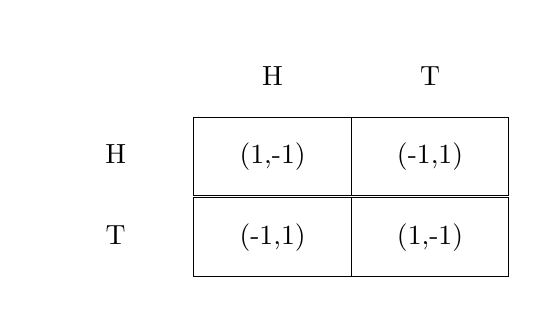
\begin{tikzpicture}[element/.style={minimum width=2cm,minimum height=1cm}]
	\matrix (m) [matrix of nodes,nodes={element},column sep=-\pgflinewidth, row sep=-\pgflinewidth,]{
		& H  & T  \\
		H & |[draw]|(1,-1) & |[draw]|(-1,1) \\
		T & |[draw]|(-1,1) & |[draw]|(1,-1) \\
	};
	
	\end{tikzpicture}
\end{center}

This results in the following instances of our definitions:
\begin{itemize}
	\item $\mathbb{S} = \{(H,H),(H,T),(T,H),(T,T)\}$
	\item $S_1 = S_2 = \{H,T\}$
	\item $u_1((H,H)) = 1$
	\item $u_2((H,H)) = -1$
\end{itemize}

\section{Pure Nash Equilibria}

Nash's key result in game theory revolved around the concept of equilibria. In simple terms, an equilibrium point in a strategic game is a strategy profile where no player can improve their payoff by just changing their own strategy. Mathematically we write:

\begin{center}
$S \in \mathbb{S}$ is a pure Nash Equilibria if $\forall i \in N, \forall s_i'$\\
$u_i(S) \geq u_i(S^{-i},s_i')$
\end{center}

We illustrate this concept by showing the pure Nash Equilibria in \textit{The Prisoner's Dilemma }
Recall the matrix form of this game:
\begin{center}
	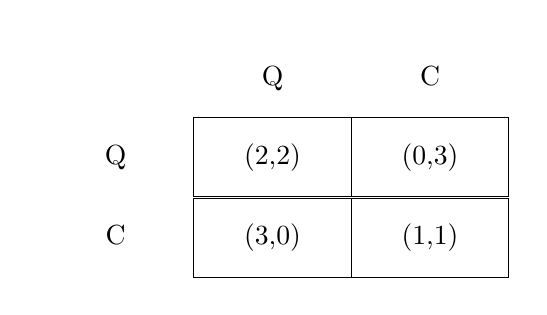
\begin{tikzpicture}[element/.style={minimum width=2cm,minimum height=1cm}]
	\matrix (m) [matrix of nodes,nodes={element},column sep=-\pgflinewidth, row sep=-\pgflinewidth,]{
		& Q  & C  \\
		Q & |[draw]|(2,2) & |[draw]|(0,3) \\
		C & |[draw]|(3,0) & |[draw]|(1,1) \\
	};
	
	\end{tikzpicture}
\end{center}

Claim: The pure strategy profile (C,C) is a pure Nash Equilibrium.

\begin{proof}
Player 1's current payoff is 2. Given that player 2 is playing pure strategy C, player 1 can only change the strategy profile to (Q,C). However, this would yield payoff of 0 for player 1 which is suboptimal. Thus, player 1 has no incentive to change their strategy. A similar argument can be made for player 2.
It is a simple exercise for the reader to check that S = (C,C) is the only pure Nash Equilibrium in this game.

\end{proof}

The Prisoner's Dilemma is a small 2-player game, but how can we check whether a strategy profile is a pure Nash Equilibrium in a larger game. To do this we introduce the concept of best response functions.\\

The idea is given the moves of the other players, what strategy will maximize player i’s utility.

\Definition Best Response Function: 
\begin{center}
	$B_i:\mathbb{S}_{-i} \Rightarrow S_i$\\
	$B_i(S_{-i}) = \{s_i \in S_i | u_i(S_{-i},s_i) \geq u_i(S_{-i},s_i') \forall s_i' \in S_i\}$
\end{center}

We can now use the best response function to prove the following theorem.

\paragraph{Theorem 1} $S^* = (s^*_1, ... , s^*_n)$ is a pure Nash Equilibrium iff $s^*_i \in B_i(S^*_{-i}) \forall i \in N$

\begin{proof}
$S^*$ is a pure Nash Equilibrium iff $\forall i u_i(S^*) >= u_i(S^*_{-i}, s_i')$ $\forall s_i' \in S_i$. iff $s^*_{-i} \in B_i(S^*_{-i})$.
\end{proof}

Using Theorem 1, we can check for pure Nash Equilibirum using best response functions. This can be done by computing the best response function value for each player for each combination of their opponent’s strategies. In a two player game, a Nash Equilibrium will just be the strategy profiles $S = (s_1, s_2)$ where $s_1 \in B_1(s_2)$ and $s_2 \in B_2(s_1)$. We illustrate this with an example.

Consider the following game:

\begin{center}
	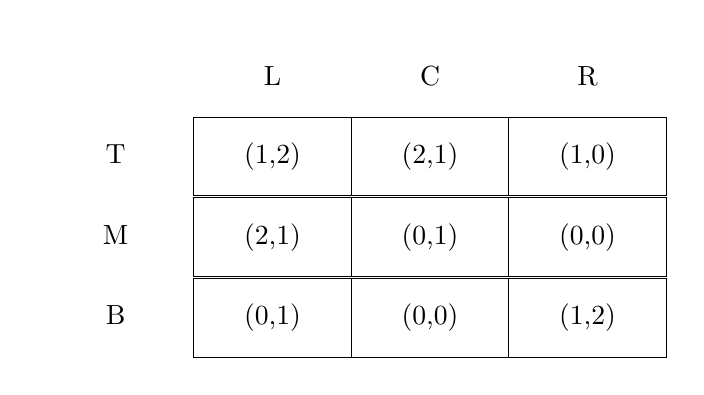
\begin{tikzpicture}[element/.style={minimum width=2cm,minimum height=1cm}]
	\matrix (m) [matrix of nodes,nodes={element},column sep=-\pgflinewidth, row sep=-\pgflinewidth,]{
		& L & C  & R  \\
		T & |[draw]|(1,2) & |[draw]|(2,1) & |[draw]| (1,0) \\
		M & |[draw]|(2,1) & |[draw]|(0,1) & |[draw]| (0,0) \\
		B & |[draw]|(0,1) & |[draw]| (0,0) & |[draw]| (1,2)\\
	};
	
	\end{tikzpicture}
\end{center}

We compute the best response functions in each case:
\begin{itemize}
	\item $B_1(L) = \{M\}$
	\item $B_1(C) = \{T\}$
	\item $B_1(R) = \{T,B\}$
	\item $B_2(T) = \{L\}$
	\item $B_2(M) = \{L,C\}$
	\item $B_2(B) = \{R\}$
\end{itemize}

It is then easy to check that $S = (M,L)$ and $S' = (B,R)$ are pure Nash Equilibria as they satisfy the requirements for Theorem 1.\\

To this point we have only considered pure Nash Equilibria. The key question is whether or not all games have such an equilibrium point. The answer in this case is no.\\

Consider again the Matching Pennies game\\

\begin{center}
	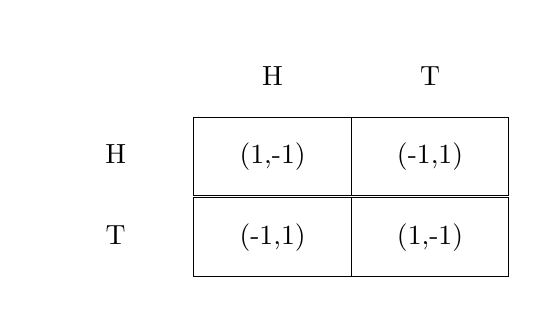
\begin{tikzpicture}[element/.style={minimum width=2cm,minimum height=1cm}]
	\matrix (m) [matrix of nodes,nodes={element},column sep=-\pgflinewidth, row sep=-\pgflinewidth,]{
		& H  & T  \\
		H & |[draw]|(1,-1) & |[draw]|(-1,1) \\
		T & |[draw]|(-1,1) & |[draw]|(1,-1) \\
	};
	
	\end{tikzpicture}
\end{center}
It is easy to see that there are no pure Nash Equilibria. If the pennies currently match, then Player 2 could change their strategy so that the pennies do not match, increasing their payoff from -1 to 1. Similarly, if the pennies do not match, player 1 can change their strategy which results in an increase of their payoff from -1 to 1. 

\section{Mixed Strategies}

As illustrated above, not all games have pure Nash Equilibria. However, we will show that all games contain an equilibrium point when we allow mixed strategies. First, we introduce the concept of mixed strategies, mixed Nash Equilibrium, and the accompanying notation.

\Definition $x^i$ is a \textbf{mixed strategy} of player $i$ which represents a probability distribution over $S_i$. We define the elements of $x^i$ as $x^i_{s_i}$ which represents the probability assigned to pure strategy $s_i$. These elements are defined for all $s_i$ in $S_i$.\\

Consistent with a probability distribution we have the following constraints on $x^i$:

\paragraph{Constraint 1:} $x^i_{s_i} \geq 0 \forall s_i \in S_i$

\paragraph{Constraint 2:} $\sum\limits_{s_i \in S_i} x^i_{s_i} = 1$\\
Compactly we write, $x^i \in \mathbb{R}^{|s_i|}_+$ with $\mathbbm{1}^T x^i = 1$\\

A pure strategy $s_i$ is simply the mixed strategy where:
\begin{equation*}
	x^i_{s_i} = 1 \text{ and }  x^i_{s'_i} = 0 | s'_i \neq s_i
\end{equation*}

We denote a mixed strategy profile as $x = (x^1, ... , x^n)$.\\ 

Our interpretation of payoff necessarily shifts to the concept of expected payoff and we overload our payoff function notation to define, in the mixed strategy framework payoff functions $u_i$ as:
\begin{center}
$u_i(X) = \sum\limits_{S \in \mathbb{S}} u_i(S)\prod\limits_{j \in N} x^j_{s_j}$\\
\end{center}
As in the pure strategy case $(x^{-i}, \bar{x}^i)$ represents the mixed strategy profile $x = (x^1, .. x^{i-1}, \bar{x}^i, x^{i+1}, ... ,x^n)$ which is the strategy profile obtained from $x$ where player $i$ has changed their strategy from $x^i$ to $\bar{x}^i$.\\

Similarly, $(x^{-i}, s_i)$ is the strategy profile where player $i$ has replaced their strategy $x^i$ with pure strategy $s_i$.\\

\newpage
The expected payoff of pure strategy $s_i$ is:
\begin{center} $u_i(x^{-i},s_i) = \sum\limits_{s_{-i} \in \mathbb{S}_{-i}} u_i(S_{-i}, s_i) \prod\limits_{j \neq i} x^j_{S_j}$\\
\end{center}

This allows us to re-write $u_i(x)$ as:

\begin{center}
$\sum\limits_{s_i \in S_i} x^i_{s_i} u_i(x^{-i},s_i)$
\end{center}
We can also redefine the concepts of equilibrium points and best response function in the context of mixed strategies as follows:

\Definition  x is a \textbf{mixed Nash Equilibrium} if $u_i(x) \geq u_i(x^{-i},\bar{x}^{-i})$ $\forall i \in N$, for all mixed strategies $\bar{x}^{-i}$ of player $i$.

\Definition Best Response Function\\
Given $x^{-i}$, the mixed strategies of all players $j \neq i$. $B_i(x^{-i})$ is the set of all mixed strategies of player $i$ with maximum expected payoff against $x^{-i}$\\

Now, we are almost ready to prove Nash’s theorem that all finite strategic games have a mixed Nash Equilibrium. First, we illustrate the idea of a mixed Nash equilibrium in the game Matching Pennies.
Recall that Matching Pennies has no pure Nash Equilibrium. We will now show that $\hat{x} = ((\frac{1}{2},\frac{1}{2}), (\frac{1}{2}, \frac{1}{2}))$ is a mixed Nash Equilibrium.

\begin{center}
	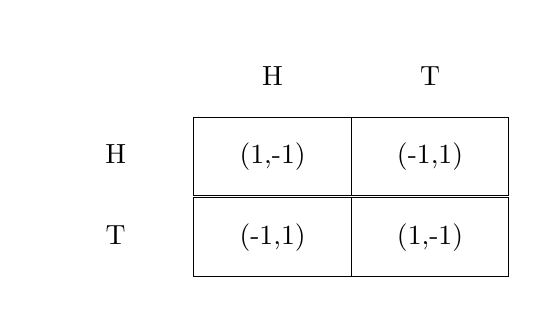
\begin{tikzpicture}[element/.style={minimum width=2cm,minimum height=1cm}]
	\matrix (m) [matrix of nodes,nodes={element},column sep=-\pgflinewidth, row sep=-\pgflinewidth,]{
		& H  & T  \\
		H & |[draw]|(1,-1) & |[draw]|(-1,1) \\
		T & |[draw]|(-1,1) & |[draw]|(1,-1) \\
	};
	
	\end{tikzpicture}
\end{center}

\begin{proof}
Let $x^1 = (\alpha, 1 - \alpha)$, $x^2 = (\frac{1}{2},\frac{1}{2})$ and $ x = (x^1,x^2)$. Then
\begin{equation*}
u_i(x) = \frac{\alpha}{2} - \frac{\alpha}{2} + \frac{(1-\alpha)}{2} - \frac{(1-\alpha)}{2} = 0 \tab \forall \alpha \in [0,1]
\end{equation*} 

$\therefore u_i((\frac{1}{2},\frac{1}{2}), (\frac{1}{2} \frac{1}{2})) \geq u_i(x^{-1},\bar{x}^{1}) \tab \forall \bar{x}^1$ mixed strategies of player 1.\\

Similarly, Let $x^* = ((\frac{1}{2},\frac{1}{2}), (\beta,1-\beta))$ where $\beta \in [0,1]$ Then,
\begin{equation*}
u_i(x^*) = \frac{\beta}{2} - \frac{\beta}{2} + \frac{(1-\beta)}{2} - \frac{(1-\beta)}{2} = 0 \tab \forall \beta \in [0,1]
\end{equation*}

$\therefore u_i((\frac{1}{2},\frac{1}{2}), (\frac{1}{2}, \frac{1}{2})) \geq u_i(x^{*-2},\bar{x}^{2}) \tab \forall \bar{x}^2$ mixed strategies of player 2. So $\hat{x}$ is a mixed Nash Equilibrium.\\ 
\end{proof}

\section{Mixed Nash Equilibrium in Finite Strategic Games}

At this point we are ready to pursue a proof of Nash's theorem that all finite strategic games contain a mixed Nash equilibrium. We will follow the method Nash used in his 1950 thesis which relies on Brouwer's Fixed Point Theorem, although Nash had previously published an alternate proof relying on the work of Kakutani. For clarity, we state Nash's theorem below:

\paragraph{Theorem 2 (Nash):} All finite strategic games contain an equilibrium point (mixed Nash Equilibrium)\\

Before proving Theorem 2, we define the results from fixed point theory that the proof relies on as well as an intermediate result which will be useful in understanding the proof.

\subsection{Definitions and Theorems from Fixed Point Theory}

\Definition X is a fixed point of a function $f: D \rightarrow D \text{ if } f(x) = x$

\Definition An \textbf{$n$-simplex}\cite{4} on $n+1$ vertices denoted $x^0,...,x^n$ is 
\begin{equation*}
x^0,...,x^n = \left \{ \sum\limits_{i=0}^n \lambda_i x^i : \forall i \in \{0,...,n\}, \lambda_i \geq 0, \sum\limits_{i = 0}^n \lambda_i = 1 \right \}
\end{equation*}

We denote a standard $n$-simplex as $\bigtriangleup_n$.

\Note The pure strategies in $S_i$ define the vertices of a $|S_i – 1|$ simplex. Every mixed strategy of player $i$ is a point within the simplex. 

\paragraph{Theorem 3 (Brouwer):} A continuous function $f: \bigtriangleup_m \rightarrow \bigtriangleup_m$ has a fixed point. That is, there exists $z \in \bigtriangleup_m$ such that $f(z) = z$.

\Note $\mathbb{S} = S_1 \times S_2 \times \cdots \times S_n$ is a convex polytope that contains all possible mixed strategy profiles (Nash)

\subsection{Support Characterization}

We now consider the structure of a mixed Nash Equilibrium $x = (x^1,..., x^n)$. Specifically, we look at the structure of each of the $x^i$’s.\\

We say that $x^i$ uses pure strategy $s_i$ if $x^i_{s_i} > 0$. We define the support of $x^i$ to be the set of pure strategies $s_i$ that $x^i$ uses.That is, $support(x^i) = \{s_i \in S_i | x^i_{s_i} > 0\}$.\\
 
Using these support sets we can characterize a mixed Nash Equilibrium using the following theorem:

\paragraph{Theorem 4 (Support Characterization):}$x$ is a mixed Nash Equilibrium iff $x^i_{s_i} > 0 \text{ only if } u_i(x^{-i}, s_i) = \max\limits_{ s_i' \in S_i} u_i(x^{-i}, s_i').$

\begin{proof}
$(\Rightarrow)$ Suppose $x$ is a mixed Nash Equilibirium and for some $s_i \in S_i$, we have $x^i_{s_i} > 0$ and $u_i(x^{-i},s_i) < \max\limits_{s_i \in S_i} u_i(x^{-i},s_i')$. Suppose $u_i(x^{-i},\bar{s}_i) = \max\limits_{s_i \in S_i} u_i(x^{-i},s_i)$. Then, we can generate new mixed strategy $\bar{x}^i$ where $\bar{x}^i_{s_i} = 0$ and $\bar{x}^i_{\bar{s}_i} = s^i_{\bar{s}_i} + x^i_{s_i}$.

Since we have just shifted probability mass from one pure strategy to another, $\bar{x}^i$ is a valid mixed strategy.\\

Consider the new utility value:\\
$\begin{array}{rl}
u_i(x^{-i},\bar{x}^i) & = \underbrace{u_i(x^{-i},x^i)}_{\text{old utility value}} - x^i_s( u_i(x^{-i},s_i)) + x^i_{\bar{s}}(u_i(x^{-i},\bar{s}_i)) = \\
& = u_i(x^{-i},x^i)+ \underbrace{x^i_{s_i}(u_i(x^{-i},\bar{s}_i) - u_i(x^{-i},s_i)}_{> 0 \text{ by assumption}})
\end{array}$\\

$\therefore$ The new utility value is strictly greater than the old value. $\therefore$ $x$ cannot be a mixed Nash Equilibrium, which is a contradiction.\\

$(\Leftarrow)$ The current utility value for player $i$ is $\max\limits_{s_i \in S_i} u_i(x^{-i}, s_i)$, as the only pure strategies with $x^i_{s_i} > 0$ have maximum expected payoff.\\

It is clear that
\begin{center} $u_i(x) = \sum\limits_{s_i \in S_i} x^i_{s_i} u_i(x^{-i},s_i) \leq \max\limits_{s_i \in S_i} u_i(x^{-i},s_i) 
\cdot \sum\limits_{s_i \in S_i } x^i_{s_i} = \max\limits_{s_i \in S_i} u_i(x^{-i},s_i)$

\end{center} as $\sum\limits_{s_i \in S_i } x^i_{s_i} = 1$ by definition.\\

$\therefore$ Player $i$ cannot increase their utility. $\therefore x$ is a mixed Nash Equlibrium.
\end{proof}

This immediately gives us the following Corollary.
\paragraph{Corollary 4:} In a mixed Nash Equilibrium $x$, $u_i(x) = \max\limits_{s'_i \in S_i} u_i(x^{-i}, s_i')$.

\begin{proof}
This is easily seen from the definition of $u_i(x)$. By Theorem 4 the only non-zero terms in the sum are those of the form $x^i_{s_i} \cdot \max\limits_{s'_i \in S_i}  u_i(x^{-i}, s_i')$. By definition, the sum of these $x^i_{s_i} = 1$, and so the whole sum is equal to $\max\limits_{s'_i \in S_i}  u_i(x^{-i}, s_i')$.
\end{proof}

\section{Proof of Theorem 2}

At this point we are finally ready to prove Theorem 2. We proceed by presenting the general idea of the proof and breaking the process down into two parts.\\

\subsection{The Idea}

The general method of this proof is to define a series of continuous linear mappings over the polytope defined by the set of mixed strategy profiles. These mapping will be designed to improve the payoff of a player if possible. However, by Brouwer's Fixed Point Theorem, the mapping will contain a fixed point. Then, all that is left to show is that this fixed point is indeed a mixed Nash Equilibrium.\\



The first portion of the proof will be dedicated to defining the mappings and showing that they satisfy the conditions of Brouwer's Theorem. The second portion will be illustrating that such a fixed point is a mixed Nash Equilibrium.

\subsection{The Proof\cite{1}} 

Given a mixed strategy profile $x$, we define the following function:

\begin{equation*}
\Phi^i_{s_i} = \max\{ 0,u_i(x^{-i},s_i) - u_i(x))\}
\end{equation*}

Clearly $\Phi^i_{s_i}$ is non-negative and $\Phi^i_{s_i} > 0$ only if $u_i(x^{-i},s_i) - u_i(x) > 0$. That is, $\Phi^i_{s_i} > 0$ only if player $i$ could increase their utility by changing strategies from $x^i$ to $s_i$.\\

$\therefore \Phi^i_{s_i} = 0$ only when $x^i$ is a best response to $x^{-i}$\\

We define $f(x) = \bar{x}$ where 
\begin{equation*}
\bar{x}^i_{s_i} = \dfrac{x^i_{s_i} +  \Phi^i_{s_i}(x)}{1 + \sum\limits_{s_i \in S_i}  \Phi^i_{s_i}(x)}
\end{equation*}

Since $ \Phi^i_{s_i}$ is continuous so is $f$.\\

We observe that the functions do not technically satisfy the conditions of the Brouwer Theorem. However, as shown by Leyton-Brown \& Shoham, Brouwer's work can be extended to Corollary 5, which we state below without proof.


\paragraph{Corollary 5:} Any continuous function $g: \prod\limits_{i \in N} \bigtriangleup_{|S_i - 1|} \longrightarrow \bigtriangleup_{|S_i -1|}$ has a fixed point\cite{4}.\\

$\therefore$ by Corollary 5, $f$ has a fixed point. It is clear to see that if $\bar{x}$ is a mixed Nash Equilibrium, then $\Phi^i_{s_i} = 0 \forall s_i$ $ \forall i$, and so $\bar{x}$ is a fixed point.\\

We show this as follows:\\

Let $\hat{x} = f(\bar{x})$. Then,
\begin{center} $\hat{x}^i_{s_i} = \dfrac{\bar{x}^i_{s_i} + \Phi^i_{s_i}(\bar{x})}{1 + \sum\limits_{s_i \in S_i}\Phi^i_{s_i} (\bar{x})} = \bar{x}^i_{s_i}$  $\forall i, s_i \in S_i$
\end{center} 
Since $\bar{x}$ is a mixed Nash Equilibrium, $\Phi_{s_i}^i (\bar{x}) = 0$ $\forall i, s_i \in S_i$. Therefore $\hat{x} = \bar{x}$\\

However, we still need to show that if $\hat{x}$ is a fixed point, then $\hat{x}$ is a mixed Nash Equilibrium. This final result is shown below:\\

Consider player $i$.\\

Let $s_i$ be in $\text{support}(\hat{x}^i)$ such that $u_i(\hat{x}^{-i}, s_i) \leq u_i(\hat{x})$. We note that $\text{support}(\hat{x}^i)$ is non-empty as $\sum\limits_{s_i \in S_i} \hat{x}^i_{s_i} = 1$. Therefore $\hat{x}^i_{s_i} > 0$ for some $s_i \in S_i$.

We now show by contradiction that there exists such an $s_i$. Assume $u_i(\hat{x}^{-i}, s_i) > u_i(\hat{x})$ $\forall s_i \in \text{support}(\hat{x})$. Let $\alpha \in \text{support}(\hat{x})$ such that $u_i(\hat{x}^{-i}, \alpha) < u_i(\hat{x}^{-i}, \beta)$ $\forall \beta \in \text{support}(\hat{x})$. Then, by definition, $u_i(\hat{x}) = \sum\limits_{s_i \in S_i} \hat{x}^i_{s_i} u_i(\hat{x}^{-i},s_i) = \sum\limits_{s_i \in \text{support}(\hat{x})} \hat{x}^i_{s_i} u_i(\hat{x}^{-i},s_i)$. The second equality sign holds as $x^i_{s_i} = 0$ $\forall  s_i \notin \text{support}(\hat{x}^i)$.

By our assumption $\sum\limits_{s_i \in \text{support}(\hat{x})} \hat{x}^i_{s_i} u_i(\hat{x}^{-i},s_i) \geq (\sum\limits_{s_i \in \text{support}(\hat{x})} \hat{x}^i_{s_i})u_i(\hat{x}^{-i}, \alpha) = 1 = u_i(\hat{x}^{-i}, \alpha) > u_i(\hat{x})$ by assumption.\\

But this is a contradiction and so there must exist $s_i \in \text{support}(\hat{x}^i)$ such that 
\begin{equation*},
u_i(\hat{x}^{-i},s_i) \leq u_i(\hat{x}_i)
\end{equation*}

Therefore $\Phi^i_{s_i}(\hat{x}) = 0$ as $u_i(\hat{x}^{-i},s_i) - u_i(\hat{x}) \leq 0$.\\

Since $\hat{x}$ is a fixed point under $f$, we have 
\begin{equation*}
\hat{x}^i_{s_i} = (f(\hat{x}))^i_{s_i} = \dfrac{\hat{x}^i_{s_i}}{1 + \sum\limits_{s_i \in S_i} \Phi^i_{s_i}(\hat{x})}
\end{equation*}
 
For this to hold, we must have
\begin{equation*}
1 + \sum\limits_{s_i \in S_i} \Phi^i_{s_i}(\hat{x}) = 1
\end{equation*}
or equivalently,

\begin{equation*}
\sum\limits_{s_i \in S_i} \Phi^i_{s_i}(\hat{x}) = 0
\end{equation*}

Since $\Phi^i_{s_i}(\hat{x}) \geq 0$ $\forall s_i \in S_i$, we must have $\Phi^i_{s_i}(\hat{x}) = 0$ $\forall s_i \in S_i$.\\

Therefore Player $i$ has no way to increase their utility. This argument works for all players $i \in N$ and therefore no player can increase their utility.

$\therefore$ $\hat{x}$ is a mixed Nash Equilibrium.
$\qed$

\newpage
\begin{thebibliography}{10}
\bibitem{1} Nash, John F.. \textit{Non-cooperative Games}.  Thesis.  Princeton University, 1950
\bibitem{2} Von Neumann, John \& Morgenstern, Oskar. \textit{Theory of Games and Economic Behaviour}. Princeton University Press. 1944.
\bibitem{3} Koenemann, \textit{CO456 - Introduction to Game Theory Course Notes}. University of Waterloo. Fall 2014.
\bibitem{4} Shoham, Yoav \& Leyton-Brown Kevin. \textit{Multiagent Systems: Algorithmic, Game-Theoretic and Logical Foundations}. 2010.

\end{thebibliography}
\end{document}